\documentclass[ProjectPlan_innit.tex]{subfiles}

\begin{document}

Our main focus with the literature review is to provide a general overview for Model Driven Development and Agile/Lean. We then intend to research further into the specifics of both areas, highlighting how they correspond or how they diverge from one another. 
\hspace{0pt} \\

The diagram (fig x) shows an overview of the main research areas that we shall be focusing upon. An initial list of literature is available in the appendix item (APPENDIX ITEM).
\hspace{0pt} \\

Literature selection shall be done based on the size and scope of the subjects, for example, we shall choose papers that cover broader areas. On the other hand, for subjects which are subsets of the broader subjects, we shall use smaller and more specific literature.
\hspace{0pt} \\

Unfortunately we are unlikely to receive much if any research materials from within Ericsson and as such we shall focus the majority of our research on external sources, journals and research papers. Our main sources of literature will be collected from popular online research repositories such as Google Scholar, The Engineering Village and the IEEE Xplore service. 
\hspace{0pt} \\

Once collected, we shall refine the literature list and sort the aggregated list based on their relevance, reliability, objectivity and usefulness to our project. 
\hspace{0pt} \\

\begin{figure*}[H!]
  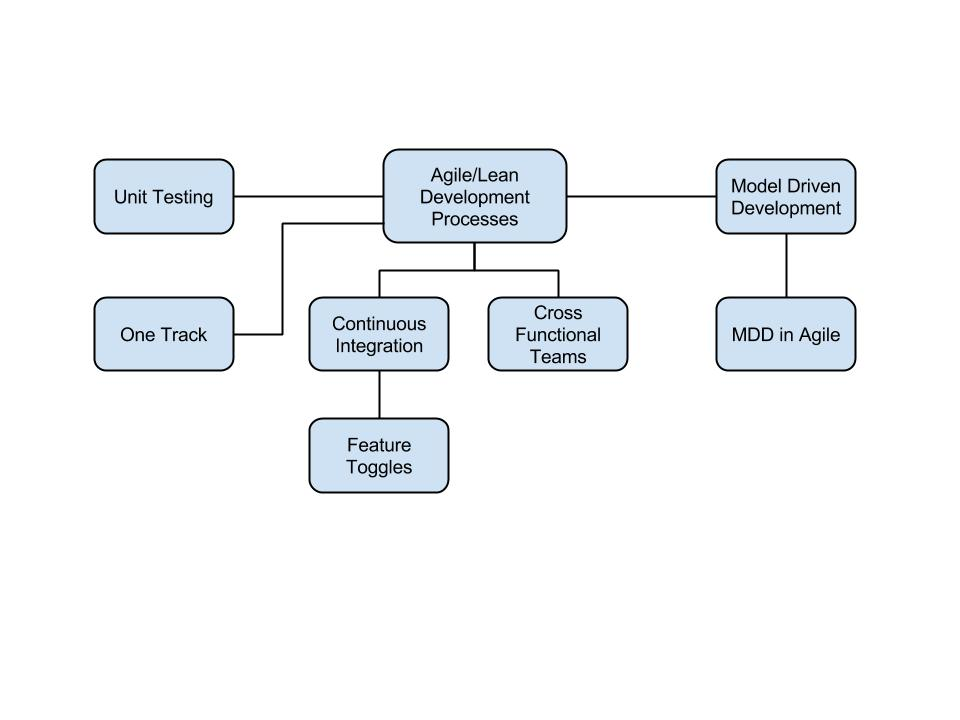
\includegraphics[width=\textwidth]{research-areas.jpg}
  \caption{Figure 2 - Mapping of research topics.}
  \label{BBB}
\end{figure*}

\end{document}